 % Author:   Gustav Tschirschnitz
% Contact:  GustavTschirschnitz@googlemail.com
% Date:     09.02.2018
% Version:  2018.0.0.2
% Description: This is a template for a thesis or a seminar paper etc. It has
% only basic functionality and tries to only incoporate up-to-date packages and
% compatbile ones. The template is designed for papers in German language. If
% you want to use this for an English thesis some things have to be changed.
% If you have questions about this template or don't know how to change stuff
% according to your needs, feel free to contact me.
% Important! You have to change the meta-data of the pdf that is going to be
% created in the style.sty (where the hyperref package is imported)
% to create a complete pdf document out of this .tex-file simply run:
% pdflatex -> biber -> pdflatex -> pdflatex
%
% Changelog:
% - 2018.0.0.1: First version of this latex template
% - 2018.0.0.2: Fixed some small typos; overhaul of the titlepage, some stuff
%               for the inclusion of a pdf file
% -----------------------------------------------------------------------------
\documentclass[12pt,a4paper,toc=chapterentrywithdots]{scrreprt}
\usepackage{tex/style} % imports the style-file which loads all the packages
\graphicspath{ {./figs/} }
\begin{document}
\hypersetup{pageanchor=false} % this disables the ability to create a link to
                              % the following pages. As we don't create a hyperlink
                              % to the titlepage or abstract (in the toc), we
                              % disable it here and enable it later on
\pagenumbering{gobble}  % disables page numbering
\subfile{tex/titlepage}
\newpage

\includepdf[pages=-]{pdfs/Aufgabenstellung Projektarbeit.pdf}
\newpage % this is needed for the page numbering to work properly. It is not
         % creating a blank page!
% put something like an abstract or a summary of the task (f.e. in form of a pdf)
% itself here (it then has no page numbering). You can do this with the command
% "\includepdf{PATH_TO_FILE}"

\pagenumbering{Roman} % page numbering is done with uppercase roman numbers
% put something like a symbol or figure directory here
\tableofcontents
\listoffigures
\listoftables
\newpage % this is needed for the page numbering to work properly. It is not
         % creating a blank page!
\hypersetup{pageanchor=true}

% \subfile{tex/00-list_of_symbols}
\newpage % this is a suggestion on how to create a list of
         % symbols. If you want to have something more like a nomenclature
         %  consider using a package for it (like nomencl or acronym)
% a list of tables and a list of figures can be created with the command "\listoftables"
% and "\listoffigures". If you want to change the heading of these paragraphs
% simple use the command "\renewcommand{\listfigurename}{Insert new heading here}"
% or "\renewcommand{\listtablename}{Insert new heading here}" before using the
% commands to create these lists
% if you want the lists to appear in the table of contents add "listof=totoc" to the
% parameters of the \documentclass{scrreprt} command

\pagenumbering{arabic} % page numbering is done with arabic numbers from now on
% -----------------------------------------------------------------------------
\subfile{tex/01-motivation}
\subfile{tex/02-grundlagen}
\subfile{tex/03-implementierung}
\subfile{tex/04-anwendung&ergebnisse}
\subfile{tex/05-schluss}

%\appendix
%\subfile{tex/AA-appendix}

%\nocite{*}
\bibliographystyle{plain}
% \bibliographystyle{apacite}
\bibliography{References}
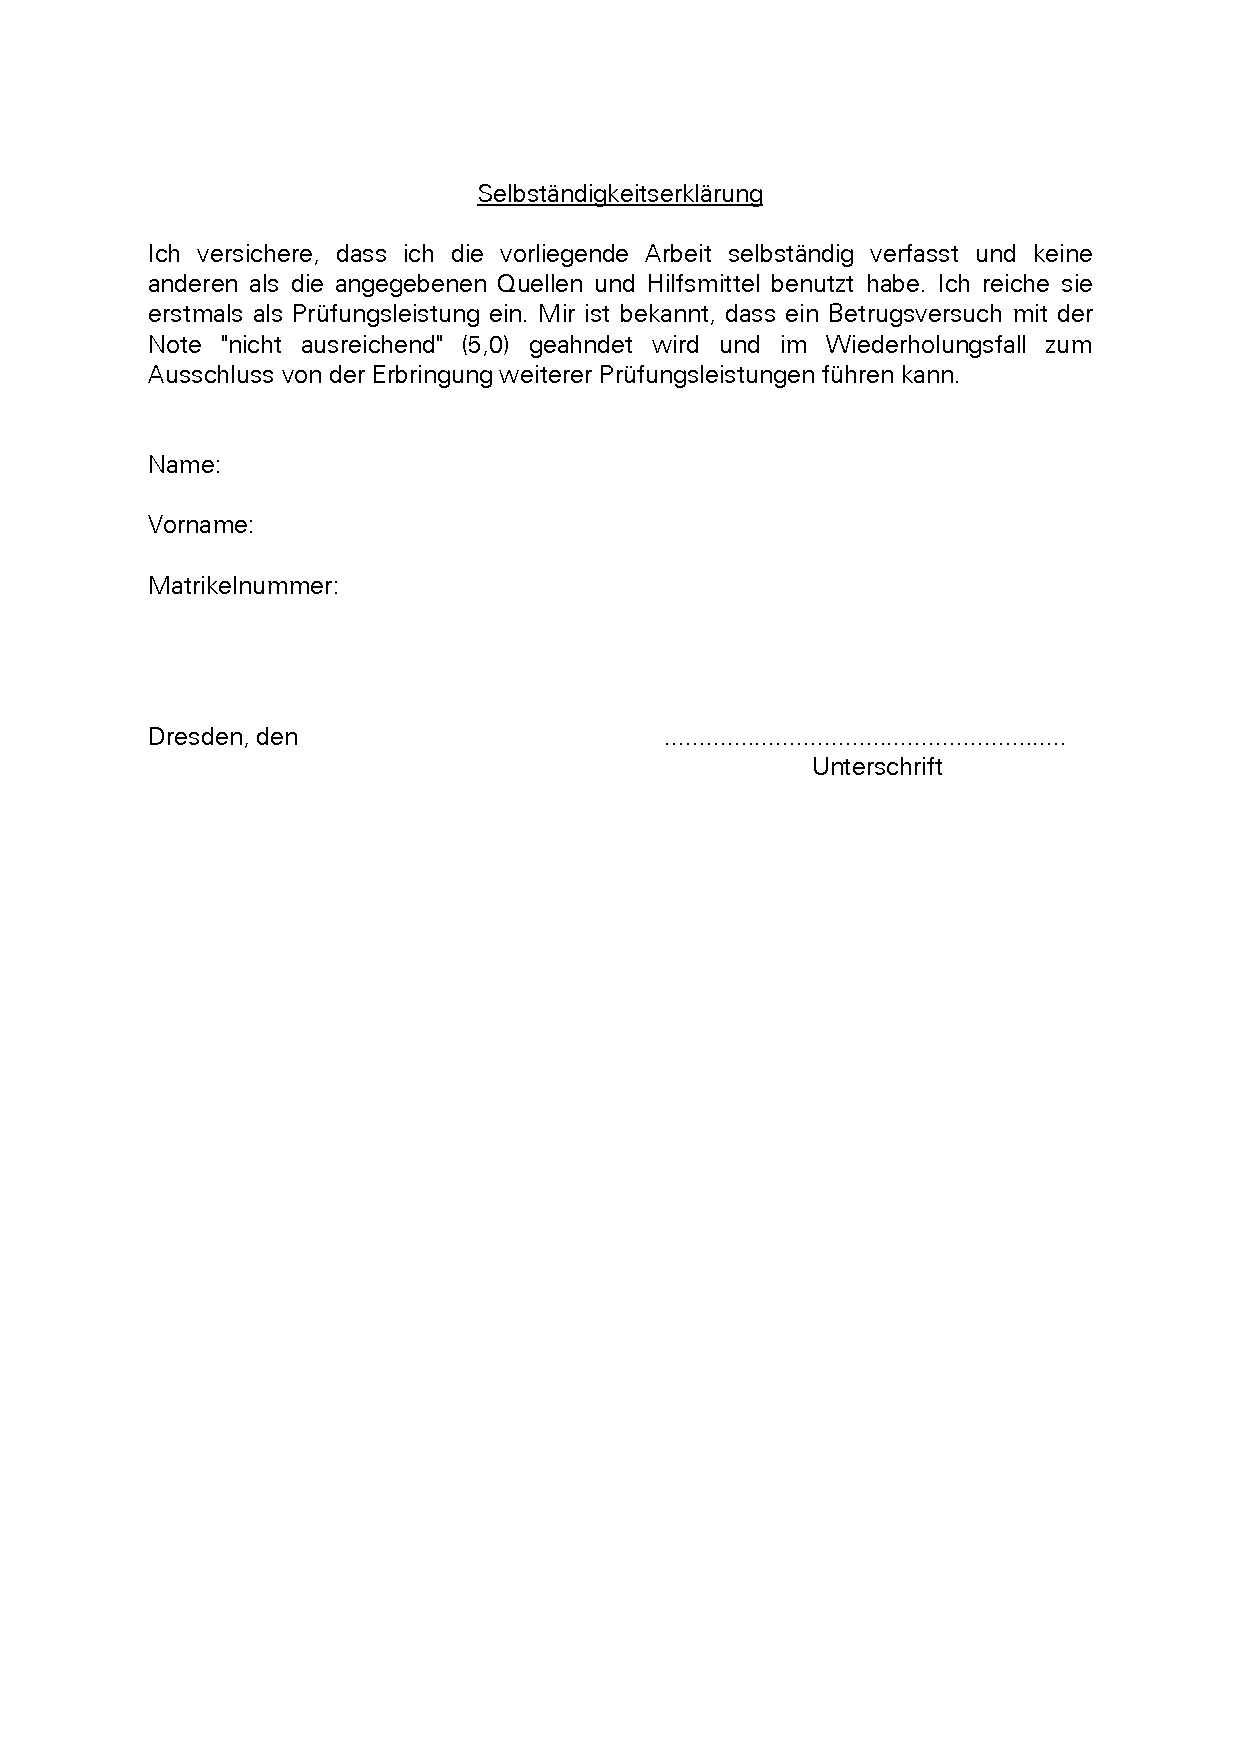
\includepdf[pages=-]{pdfs/Selbststaendigkeitserklaerung.pdf}
\end{document}
